\documentclass[tikz,border=0pt]{standalone}
\usepackage{xcolor}
\definecolor{timblue}{RGB}{0,0,255}
\begin{document}
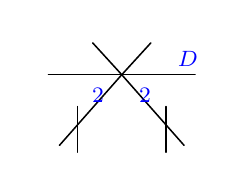
\begin{tikzpicture}[x=1pt,y=-1pt,line width=0.55pt,line cap=round,line join=round]
  \path[use as bounding box] (0,0) rectangle (67.992,47.56);

  % Exact line coordinates from the accepted IX-1 SVG.
  \draw (7.5,17.0) -- (60.5,17.0);
  \draw (23.5,5.5) -- (34.0,17.0);
  \draw (44.5,5.5) -- (34.0,17.0);
  \draw (34.0,17.0) -- (11.5,42.5);
  \draw (34.0,17.0) -- (56.5,42.5);
  \draw (18.0,28.5) -- (18.0,45.0);
  \draw (50.0,28.5) -- (50.0,45.0);

  \node[anchor=base west,inner sep=0pt,text=timblue,font=\fontsize{8.5}{9}\selectfont]
    at (23.0,27.0) {$2$};
  \node[anchor=base west,inner sep=0pt,text=timblue,font=\fontsize{8.5}{9}\selectfont]
    at (40.0,27.0) {$2$};
  \node[anchor=base west,inner sep=0pt,text=timblue,font=\fontsize{8.5}{9}\selectfont]
    at (54.0,14.0) {$D$};
\end{tikzpicture}
\end{document}
